\documentclass{report}
\usepackage{suthesis}
\usepackage{amsmath}
\usepackage{graphicx}

\dept{Music}

\begin{document}
\title{Mathematical models of rhythm synchronization and anticipation}
\author{Iran R. Roman}
\principaladviser{Chris Chafe}
\firstreader{Edward W. Large}
\secondreader{Julius O. Smith}

\beforepreface

\prefacesection{Abstract}
When humans synchronize with a periodic stimulus, endogenous processes like neural delays and spontaneous rates can explain the systematic asynchronies observed between human movements and stimulus onsets. This dissertation presents two different models that explain how neural delays and spontaneous rates of movement affect human synchronization. Additionally, these models have been implemented with tensorflow 2, allowing for parameter optimization and general applications in signal processing algorithms.
The first model explains how, in metronome synchronization tasks, people tend to tap slightly before the metronome clicks. This anticipation tendency increases with longer stimulus periods of up to 3500ms, but is less pronounced in trained individuals like musicians compared to non-musicians. In non-biological systems, anticipation is observed between delayed-coupled systems. Therefore, the human anticipation tendency could be explained with such a system because delayed communication is inherent to the sensorimotor system during perception-action coordination. This dissertation tests this hypothesis with a dynamical systems model consisting of an oscillator receiving its own delayed activity as input. Simulation experiments were conducted using previously published behavioral data from human studies with either synchronization to a metronome or interpersonal synchronization. Our new model is validated by its ability to simulate real human synchronization and anticipation data. As a result, our model informs theories of adaptive human synchronization.
The second model explains how interpersonal synchronization is affected by an individual’s spontaneous rates of movement. Specifically, the greater discrepancy between two synchronizing musicians' spontaneous rates, the greater asynchronies observed during joint duet performance. Interestingly, a musician's spontaneous rate remains stable after experiencing a joint performance, suggesting short-term tempo adaptation during joint performance and spontaneous rate restoration afterwards. This dissertation tests whether an oscillatory dynamical system with frequency elasticity and hebbian learning can explain how spontaneous rates affect interpersonal synchronization. The model consists of an oscillator with a natural frequency that emulates the human spontaneous rate. The oscillator’s frequency term is elastic to allow for short-term frequency changes during synchronization with a periodic stimulus of an arbitrary frequency. However, elasticity makes the oscillator return to its original natural frequency when it is no longer stimulated. Our model is validated by its ability to simulate human synchronization data using its adaptive and elastic frequency learning mechanism. This model can simulate duet musical performance and explain how asynchronies between performers are systematically influenced by the difference between two performers’ spontaneous rates.
Finally, this dissertation presents a novel implementation of these oscillatory models in tensorflow 2. This toolbox is written with a broad user-base in mind, and it includes general numerical methods for integration of ordinary differential equations. Besides allowing users to simulate different types of neural oscillators in multi-scale networks, the toolbox also allows oscillatory models to be combined with deep learning networks for the first time. Oscillatory networks are a new alternative for time-frequency analysis in deep learning algorithms, and can improve performance in common signal processing tasks.

\prefacesection{Acknowledgments}
I would like to thank my colleagues, family, and friends. Thank you to my CCRMA cohort of Ph.D. candidates: Kitty Shi and Tim O'Brien. Similarly, I want to thank all the friends I had at CCRMA: Madeline Huberth, Alex Chechile, Wisam Reid, Shu Yu Lin, Nick Gang, Ethan Geller, Rahul Agnihotri, Emily Graber, John Granzow, Woody Herman, Kai-Chieh Huang, Jay Kadis, Sasha Leitman, Sara Martı́n, Romain Michon, Kitty Shi, Dave Kerr, Fernando Lopez-Lezcano, Carr Wilkerson, Elliot Kermit-Canfield, Eoin Callery, Jorge Herrera, Rob Hamilton, Chryssie Nanou, Christopher Jette, Matt Wright, Nette Worthey, Mario Champagne, Velda Williams, and Debbie Barney. Outside of CCRMA, I want to thank the Bioscience community: Samar Fahmy, Terrance Mayes, Tim Stearns, Ayodele Thomas, and Tony Ricci. 
A big thank you to the Stanford Human-Centered Artificial Intelligence initiative for funding the last year of my Ph.D. studies, and the Howard Hughes Medical Institute for funding my first academic quarter at Stanford. 
I also want to thank CCRMA faculty. Thank you Malcolm Slaney and Takako Fujioka for providing critical feedback and advice to my modeling work presented in this dissertation. Thanks for Jonathan Abel and David Berners for letting me serve as their teaching assistant of signal processing. Thank you Jonathan Berger and Jaroslaw Kapuscinski for always being supportive and providing me with general academic advice. Thank you Ge Wang for your courses where I learned the fundamentals of algorithms applied to digital sound. 
My dissertation committee deserves a big thank you for all their work guiding my Ph.D. research. Thank you Julius Smith for inspiring me to always extend my horizons and for being an excellent role model of scholarship and creative thinking. Thank you Edward Large for always being supportive of my research efforts and guiding me whenever I felt lost. And thank you to Chris Chafe for trusting in my ideas and letting me shape my research agenda. 
My journey at Stanford was possible thanks to the support that my family gave me. Thank you Alejandra Torres for being the most caring and sincere individual I have ever met, and thank you for always being there. Thank you Iran A. Roman for bringing joy to all my days. I also want to thank my supportive and loving parents: Adriana Guzman Guzman and Iran Manuel Roman Jaimes. Finally, thank you to my brothers Rodolfo, Rodrigo, and Adrian.
\afterpreface

\chapter{Introduction}
Humans perform rhythm actions everyday. As individuals, we carry out spontaneous rhythmic movements like walking or blinking. We also can perform movements that are paced by an external stimulus, like tapping our foot while listening to music. And we also perform rhythmic actions interpersonally, with others, for example when we play or sing music together.
These rhythmic actions are periodic; affected by internal factors, meaning that they are different between people (that’s why two pianists play the exact same tune differently); they are also affected by external factors, meaning that one’s environment can affect how we perform these actions (that’s why the same guitarist may play differently with different bands). This dissertation aims at explaining how internal and external factors affect human rhythmic action. And the methodology to do that will consist of simulating human rhythmic actions with simple oscillatory equations and other physical principles. 
How can we simulate human rhythmic actions? In the work presented here we used a dynamical systems equation that oscillates like a sinusoid. This oscillator shows spontaneous periodic activity, which can be used to simulate human periodic actions. This equation can also be driven by an external stimulus (here indicated by the F term at the end of the equation). When stimulated with a periodic signal, this oscillator can show stable synchronization or unstable activity, depending on the frequency difference between the oscillator’s natural frequency and the stimulus frequency. In this plot, a frequency difference around zero results in stable synchronization anticipating or lagging the stimulus. But as the frequency difference becomes larger, unstable behavior is observed. Humans can synchronize and anticipate stimuli of multiple frequencies. Therefore, to simulate human rhythmic action we will need to use two other physical principles. The first one is strong anticipation, which, as its name indicates, states that physical systems with delayed feedback show anticipatory behavior. In this plot the dotted sinusoid anticipated the other because of strong anticipation. The second one is frequency elasticity, which explains how an oscillator can adaptively change the frequency of its sinusoidal activity. In this plot you see an oscillator’s frequency, represented by a solid line, moving from one initial value to another one represented by the dotted line. Later on I will explain all these concepts in detail, but I am mentioning them now to state what the research goals of my PhD project were, as well as their significance. 
How can we simulate human rhythmic actions? In the work presented here we used a dynamical systems equation that oscillates like a sinusoid. This oscillator shows spontaneous periodic activity, which can be used to simulate human periodic actions. This equation can also be driven by an external stimulus (here indicated by the F term at the end of the equation). When stimulated with a periodic signal, this oscillator can show stable synchronization or unstable activity, depending on the frequency difference between the oscillator’s natural frequency and the stimulus frequency. In this plot, a frequency difference around zero results in stable synchronization anticipating or lagging the stimulus. But as the frequency difference becomes larger, unstable behavior is observed. Humans can synchronize and anticipate stimuli of multiple frequencies. Therefore, to simulate human rhythmic action we will need to use two other physical principles. The first one is strong anticipation, which, as its name indicates, states that physical systems with delayed feedback show anticipatory behavior. In this plot the dotted sinusoid anticipated the other because of strong anticipation. The second one is frequency elasticity, which explains how an oscillator can adaptively change the frequency of its sinusoidal activity. In this plot you see an oscillator’s frequency, represented by a solid line, moving from one initial value to another one represented by the dotted line. Later on I will explain all these concepts in detail, but I am mentioning them now to state what the research goals of my PhD project were, as well as their significance. 

\chapter{Delayed feedback embedded in perception-action coordination cycles results in anticipation behavior}
\chaptermark{Delayed feedback results in anticipation behavior}

\section{Introduction}
In social settings, people must coordinate actions in order to carry out fundamental activities like walking or talking. Some activities require individuals to precisely time repetitive actions such as dancing, rowing, or music making, resulting in synchronization with external information, shared among a group of individuals. This kind of perception-action coordination is also sometimes called sensorimotor synchronization, because it is considered to depend on communication between the sensory and motor areas of the nervous system \cite{oullier2005neural}. The simplest form of synchronization happens when individuals tap in synchrony with an isochronous stimulus. In doing so, individuals’ actions on average tend to slightly precede the stimulus, resulting in a mean negative asynchrony between the stimulus onsets and corresponding taps. This negative mean asynchrony has been observed consistently in the literature. Anticipation is observed when humans tap with an isochronous stimulus with inter-onset-intervals (IOIs) ranging from 300ms to 4800ms \cite{mates1994temporal}. However, the asynchronies vary widely and can be positive, on average, for an individual tapping with IOIs longer than 2000ms \cite{mates1994temporal}. For IOIs greater than 2000ms, asynchronies may show a bimodal distribution; some taps precede the stimulus while others follow it, with longer IOIs resulting in more taps that follow the stimulus and fewer that precede it \cite{baaaath2016estimating}. The anticipation tendency is influenced by musical experience, as tap timing in musicians is closer to the stimulus than that in non-musicians for IOIs between 1000ms and 3500ms \cite{repp2007tapping}. When the IOI is greater than 5000ms, more taps occur after the stimulus than before the stimulus, suggesting that people are more reactive upon hearing the next beat \cite{miyake2004two}. Similarly, when synchronizing with the beat underlying complex surface rhythms (e.g., syncopation), the mean asynchrony shifts to the positive side \cite{wohlschlager1999synchronization, snyder2001tapping, large2015neural} (see \cite{repp2005sensorimotor} for a review). Collectively, these results indicate that the anticipation tendency depends not only the IOI, but also, the expertise level, complexity of the rhythms and the task requirements.

Two or more people can also perform coordinated rhythmic behavior. For example, two musicians may alternate taps to maintain a common stable tempo. To achieve coordination, they must employ an interactive and adaptive strategy and adjust their tap timing based on their own timing as well as their partner's. The asynchrony of one person tends to copy the previous asynchrony produced by their partner \cite{nowicki2013mutual, konvalinka2010follow}. This tendency is not observed when one of the partners cannot hear the actions of the other, indicating that the auditory feedback between synchronizing partners can affect their ability to coordinate \cite{palmer201210}. It appears that in the presence of auditory feedback, coordination is not affected by the presence or absence of other non-auditory information \cite{nowicki2013mutual, marmelat2012strong}. Another factor that affects auditory information in coordination is transmission latency (TL), which refers to a delay between the time at which an event occurs and the time when the associated auditory information is available. TLs are a result of the transmission of information across a physical distance separating two synchronizing individuals \cite{chafe2010effect}. Analogous latencies can be observed when musicians at remote locations play music together over the internet. One study has examined the effect of the TL between two individuals trying to alternately clap a rhythm \cite{chafe2010effect}. The authors observed that stable synchronization is achieved with small TLs (10-20ms), while musicians collectively speed up for TLs shorter than 10ms, and slow down for latencies longer than 20ms \cite{chafe2010effect}.

Different models try to explain how neural computations give rise to anticipation and coordination. Researchers have proposed that the anticipation results from the combination of information from different modalities, based on differences in the axonal distances between the hand, the ear, and the brain \cite{aschersleben1995synchronizing, prinz1992don}. For example, the sensory accumulation model \cite{aschersleben2002temporal} proposes that the time difference in central-peripheral signal communications between the auditory and motor systems may be responsible for the anticipation; it takes less time for pacing stimuli to travel from the ear to the auditory cortex compared to the time it takes a signal to travel from the fingertips to the brain and vice versa. As a result, taps precede external auditory signals so somatosensory and auditory information will coincide at the level of the central nervous system. One prediction of the sensory accumulation model is that louder stimuli will result in smaller anticipation. Białuńska, Bella, \& Jaśkowski tested this theory behaviorally, and found that the prediction was not confirmed, indicating that other sensorimotor mechanisms must be involved \cite{bialunska2011increasing}. Another model proposes perceptual underestimation of IOIs \cite{flach2005transition}. This predicts that anticipation should be reduced when periodic stimuli are subdivided into equidistant strong and weak beats \cite{loehr2009subdividing, repp2008metrical, zendel2011effects}. However, due to conflicting results, an integrative and convergent explanation is still yet to be established (see \cite{repp2013sensorimotor} for a review).

Mechanisms underlying generalized anticipatory behavior beyond the simple anticipatory phenomena have recently been of interest. Dubois \cite{dubois2001incursive} has identified two main theories as to how anticipatory behavior arises. The first one is called ‘weak anticipation theory’, proposing that anticipation occurs as the result of inferences produced by internal models. Specifically, this theory argues that because the brain generates representations of likely future events based on external information, anticipation is the result of the brain’s eagerness to confirm the correctness of these representations \cite{clark1998being, clark1999towards}. The second perspective is termed ‘strong anticipation theory’, which suggests that anticipation results from the homeostatic coupling of information between an organism and its environment. Stepp and Turvey \cite{stepp2010strong} note that, in its original Latin meaning, anticipation refers to the act of “following a path before.” Accordingly, anticipation must involve not only correctly predicting another model’s actions but also realizing that prediction with one’s own actions \cite{stepp2010strong}. Stepp and Turvey also explained that homeostatic mechanisms can keep an anticipating organism in a proactive state \cite{stepp2010strong}. One can see that a major drawback of the weak anticipation theory is that it cannot explain how some physical systems anticipate, even without the ability to carry out inference (e.g., laser semiconductors and electronic circuits) \cite{washburn2015harmony, kelso1995dynamic}. In contrast, strong anticipation theory can explain anticipation as a theoretical framework that generalizes across physical systems \cite{stepp2010strong}. The present study is aimed at exploring how the strong anticipation theory could further explain various results in rhythmic coordination in an integrative manner, including anticipatory synchronization, by conducting computational simulations.

Specifically, ‘anticipatory synchronization’ in strong anticipation emerges from the coupling between a 'response' system and a 'driver' system (e.g., stimulus input) wherein the response system also receives delayed feedback about its own activity. One of the major strengths of the strong anticipation approach is that it accounts for anticipatory phenomena beyond human behavior, and that collectively all such phenomena can be modeled as coupled dynamical systems \cite{stepp2010strong, washburn2015harmony, kelso1995dynamic}. There are parallels between a dynamical system with delayed feedback and the delayed communication between different areas in the sensorimotor system of humans carrying out synchronization. Synchronization requires communication between auditory, premotor and motor brain areas \cite{merchant2015finding, banerjee2007neural, slowinski2016effects}, which involves delayed transmission of neural information. Moreover, it has been suggested that these delays inherent within the human sensorimotor system may act like ones in coupled dynamical systems with delayed feedback inputs \cite{washburn2015harmony, banerjee2007neural, slowinski2016effects}, supporting the strong anticipation theory. If this holds true, a low-dimensional dynamical systems model could explain anticipation in perception-action coordination.

To simulate periodic perception-action coordination, we use an oscillator described by Eq \eqref{eq:2.4} (see model definition in the methods section). This oscillator can synchronize with periodic external stimuli, a feature that has been exploited by a model capable of beat tracking in complex musical rhythms \cite{large2015neural, velasco2011pulse}. The oscillator’s periodic activity phase-locks with external periodic stimuli close to its fundamental frequency and also at integer-ratio relationships \cite{large2010canonical}.

In contrast to the models previously described by Large and colleagues using a network of coupled oscillators \cite{large2015neural, velasco2011pulse, large2010canonical}, our model consists of a single oscillator. To simulate periodic synchronization, we add delayed recurrent feedback to this single oscillator. Such delayed recurrent feedback is essential for a model of synchronization, as no neural process is instantaneous \cite{banerjee2007neural}. We refer to our model as the Strong Anticipation in Periodic Perception Action (SAPPA) model (see model definition in the methods section). Below we describe three simulation experiments (see Fig \ref{f2_1}) based on published data corresponding to three distinct behavioral studies.

\begin{figure}[!h]
    \centering
    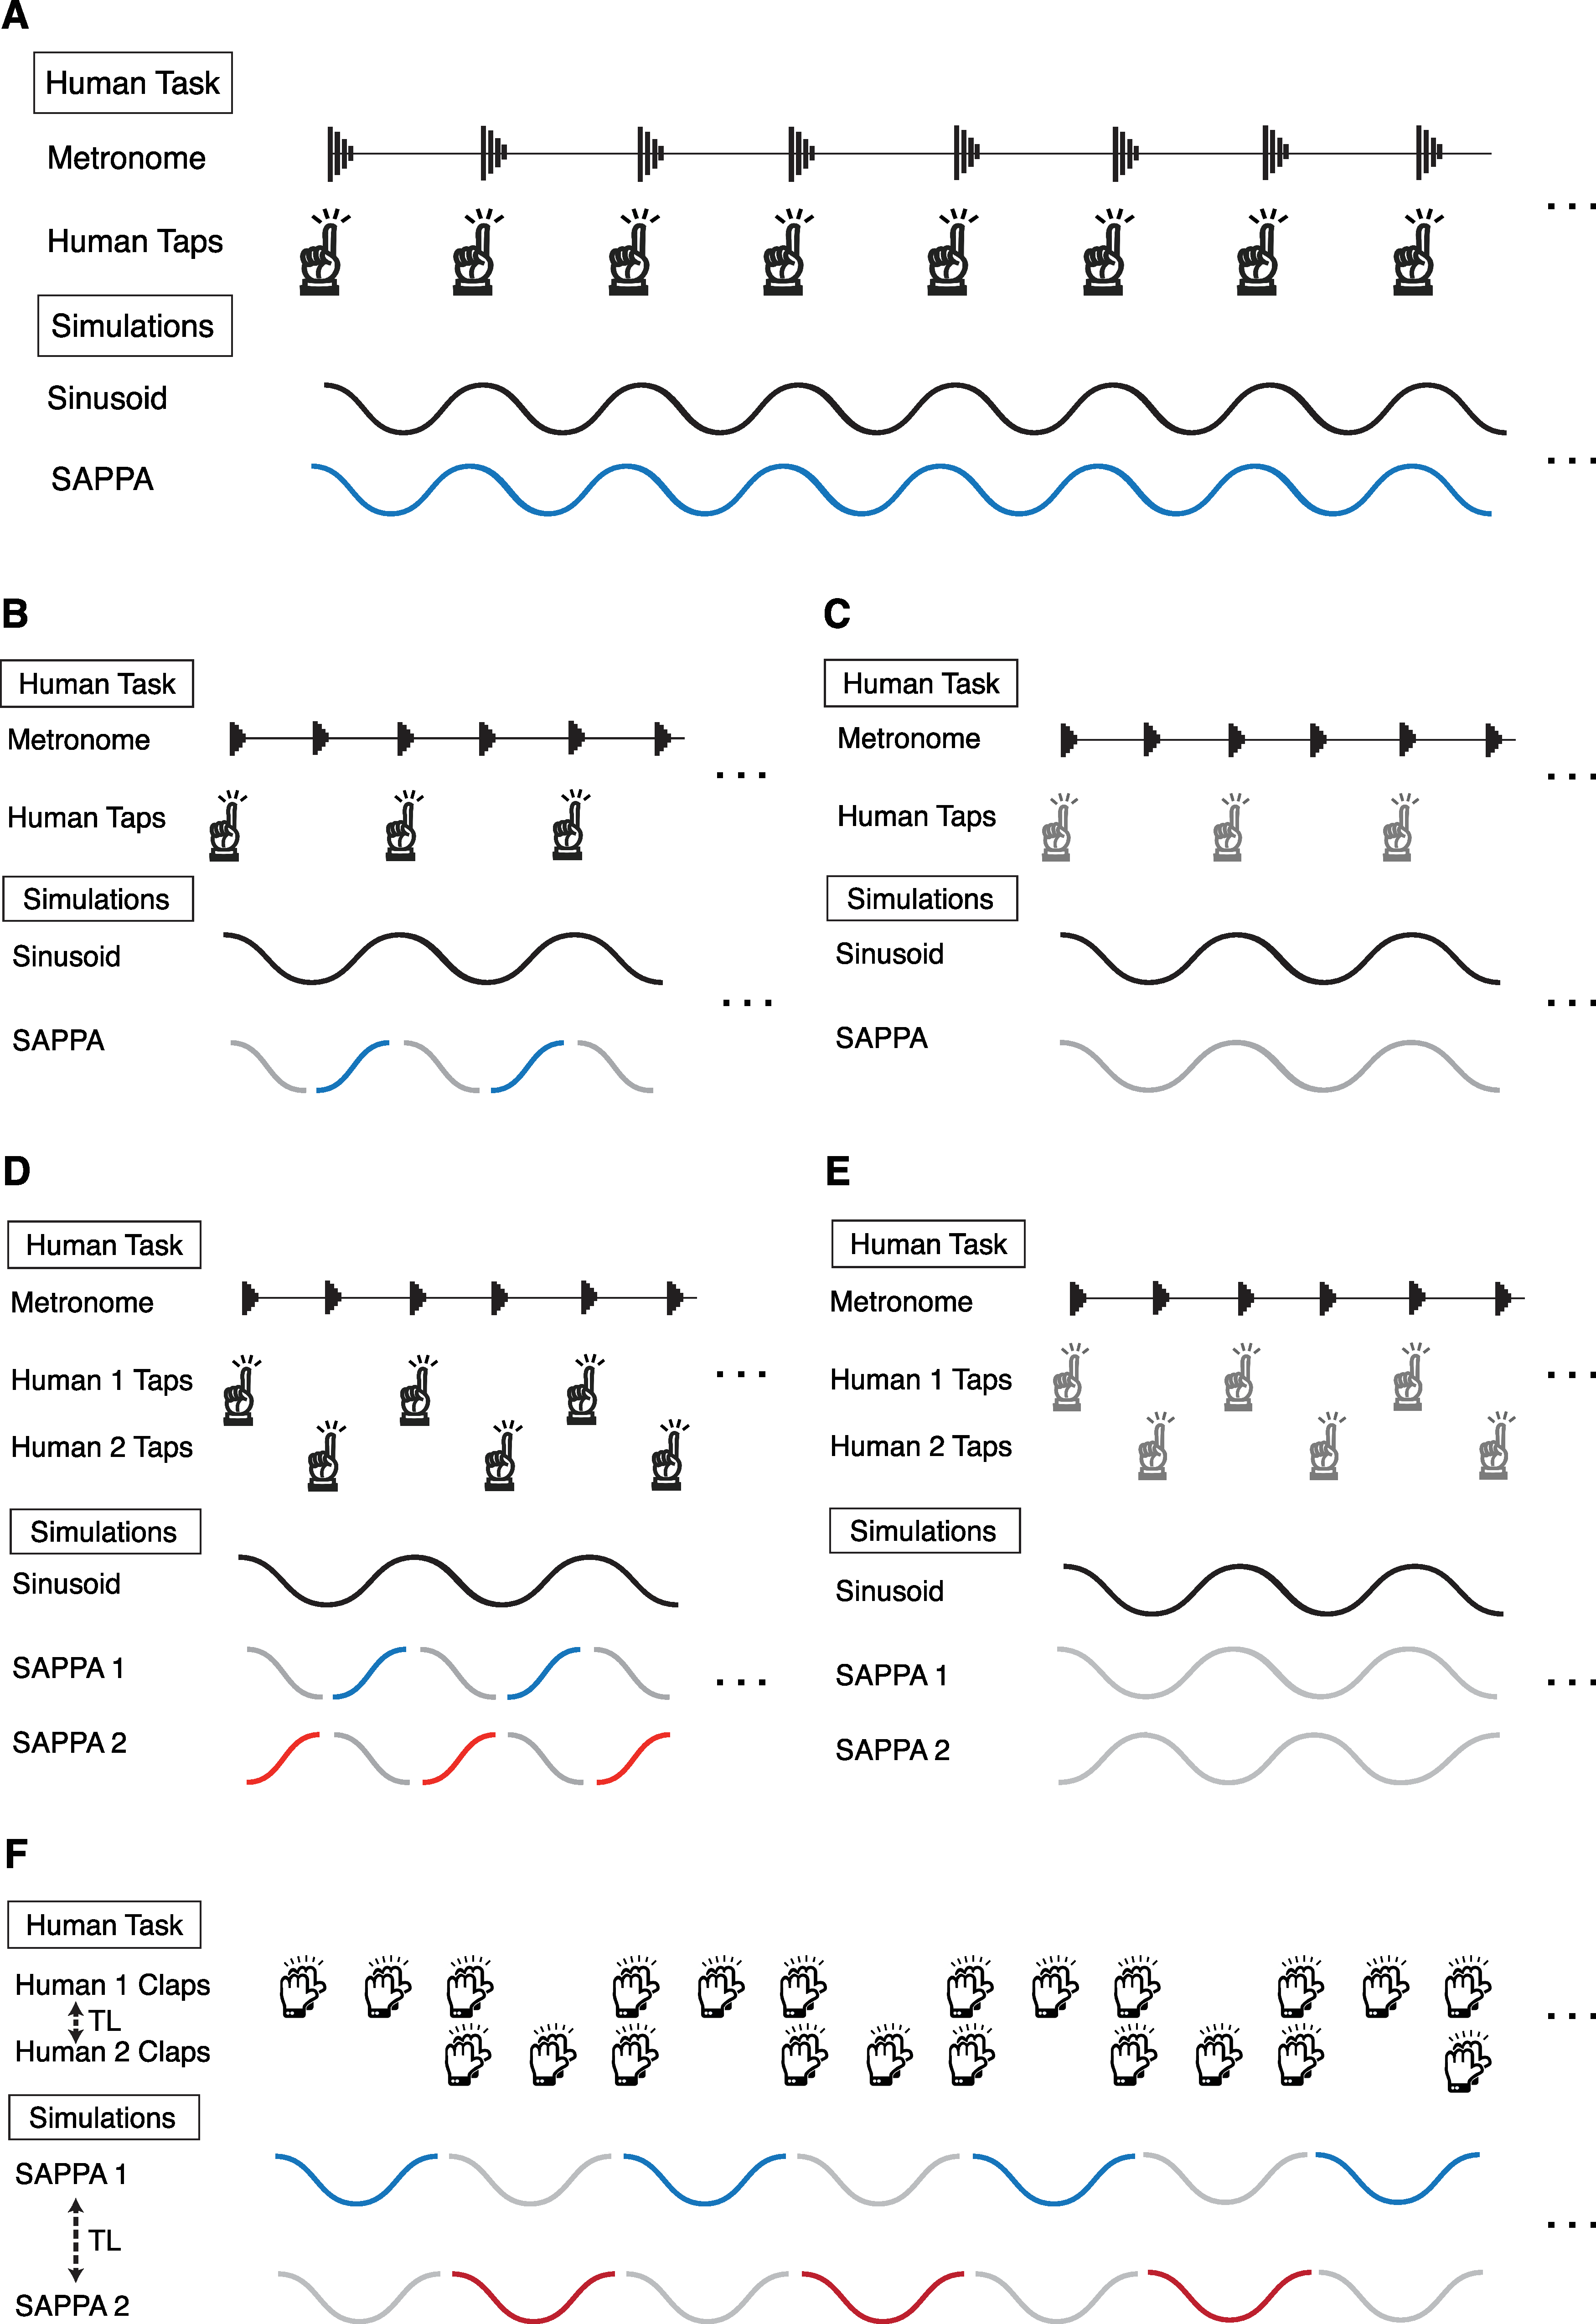
\includegraphics{figures/fig2_1.png}
    \label{f2_1}
\end{figure}
\begin{figure}[!h]
    \caption{\textbf{Illustration of the synchronization tasks and corresponding simulation experiments.} (A) The task simulated in Experiment 1, in which a person synchronizes with a metronome (top). Illustration of our simulation, in which our model synchronizes with an external sinusoidal stimulus (bottom). (B) The first task simulated in Experiment 2, in which one musician taps to every other metronome beat while listening his or her own taps (top). Illustration of our simulation in which a SAPPA model synchronizes with an external sinusoidal stimulus (bottom). Blue colored part of the model’s activity indicates that the model is receiving its own non-delayed activity as input in addition to the external sinusoid, and gray colored part indicates that the model only receives the external sinusoid as input. (C) The second task simulated in Experiment 2. This task is the same as the first one described in (B), except that the musician did not hear his or her own taps (top). Illustration of our corresponding simulation (bottom). The gray lines indicate that the model only receives the external sinusoid as input. (D) The third task simulated in Experiment 2, in which two musicians alternately tap with a metronome while listening to their own taps and the other musician’s taps (top). Illustration of our simulation where two models synchronize with an external sinusoidal stimulus (bottom). Blue and red colored parts of the model’s activity indicate the time window where the model’s non-delayed activity is used as input for both models in addition to the external sinusoid, while grayed part indicates the time window when the model receives the non-delayed activity of the other model in addition to the external sinusoid as input. (E) The fourth task simulated in Experiment 2. This task is the same as the third one described in (D), except that the musicians did not hear their own or each other’s taps (top). Illustration of our corresponding simulation (bottom). The grayed cycles indicate that the models only receive the external sinusoid as input. (F) The task simulated in Experiment 3, in which two musicians clapped a rhythm alternately (top). Illustration of our simulation where two models oscillate while alternately receiving each other’s activity as input (bottom). Blue and red cycles indicate the model whose activity is received by both models as input, while gray cycles indicate that the model’s activity is not received as input by either model. TL stands for transmission latency.}
\end{figure}

In our first experiment, we use the SAPPA model to reproduce the data from a study in which musicians and non-musicians synchronized their tapping with an isochronous metronome across a wide range of tempi, representing the simplest form of synchronization task [4] (Fig 1A). Specifically, we hypothesize that the delayed recurrent feedback in the SAPPA model would result in an increasing anticipation tendency for the longer stimulus periods. Additionally, the smaller anticipatory tendency observed in musicians compared to non-musicians’ anticipatory tendency would be achieved by reducing the amplitude of the delayed recurrent feedback.

In our second experiment, we reproduce the data from a study in which two musicians alternately tapped to a metronome [12]. We are specifically interested in the data from two tasks where musicians tapped at every second metronome beat alone (Fig 1B and 1C) or alternated this tapping with another musician as a duet (Fig 1D and 1E). In both cases, their performance was measured in two conditions, with and without auditory feedback from tapping. The results show a smaller anticipatory tendency, in both solo and duet settings, when musicians heard their own taps compared to when they did not. We hypothesized that the lack or presence of non-delayed feedback in our model can simulate auditory feedback conditions, affecting the size of the anticipation.

In our third experiment, we reproduce behavioral data from duet performance with TLs (varying from 3ms to 78ms for different trials) where two musicians alternately clapped the same rhythmic pattern without a metronome [14] (Fig 1F). Latencies longer than 20ms caused the musician starting the pattern to lag the musician finishing the pattern, while latencies shorter than 10ms caused the musician starting the pattern to clap ahead of the other musician’s last clap. This resulted in the collective tempo gradually slowing down for the longer TLs and speeding up for the shorter ones. We hypothesized that our model’s anticipation would be affected by longer TLs, resulting in lag between two synchronizing SAPPA models and a slowing tempo.

Perception-action coordination tasks capture how external and internal factors affect synchronization. The strong anticipation hypothesis explains synchronization with dynamical systems receiving external stimuli and delayed recurrent feedback. Our interest is to test whether a mathematical model of strong anticipation can be configured for solo and duet settings to perform a variety of synchronization tasks, and if so whether it could explain behavioral patterns observed in human data. This would demonstrate that the strong anticipation hypothesis accounts for complex biological phenomena like perception-action coordination.

\begin{equation}
\frac{1}{f}\dot{z} = z\bigg(\alpha + i2\pi + \beta_1|z|^2 + \frac{\epsilon\beta_2|z|^4}{1-\epsilon|z|^2}\bigg) + F \label{eq:2.4}
\end{equation}


\chapter{Hebbian tempo learning with elasticity explains how a musician's spontaneous motor tempo affects periodic synchronization}
\chaptermark{Hebbian learning explains synchronization}

\section{Introduction}
Humans can seamlessly sing a song in the shower or walk on an empty street. In such a solo setting, individuals show a spontaneous singing tempo or walking pace. In everyday life, however, humans often have to synchronize with external signals. For example, singing with a pre-recorded song or marching in a parade with other individuals. In the specific case of musical performances, musicians change the tempo of their actions to match a predetermined musical tempo that is kept by the group of performing musicians. When musicians synchronize with each other they carry out perception-action coordination (PAC), which involves the coordinated communication between the brain’s sensory areas that perceive stimuli and the motor system that executes actions (Ridderinkhof and Ridderinkhof, 2014). It is obvious that most musical performances will not match a musician's spontaneous tempo. However, how a musician's spontaneous tempo affects a musical performance is still an open question (Zamm et al., 2016). To tackle this question, one must first study an individual’s spontaneous tempo of periodic action, like finger tapping. The spontaneous motor tempo (SMT) can be obtained by calculating the average inter-onset interval (IOI) between consecutive periodic actions, usually in milliseconds (McAuley et al., 2006). SMTs vary within individuals, tending to be shorter in early childhood compared to adulthood (McAuley et al., 2006), and between individuals, tending to be longer in adult musicians (~400ms IOI on average) compared to non-musicians (~300ms IOI on average) (Scheurich et al. 2016; Drake et al., 2000).

\chapter{Motivations to combine delayed feedback and Hebbian elastic frequency learning}
\chaptermark{Delayed feedback and Hebbian learning}
The next step would be to combine the anticipation and elastic frequency learning models that we have talked about today. Although that goes beyond the scope of this dissertation, this would let us answer questions like: How are axonal delays and endogenous rhythms related to each other? Why is the negative mean asynchrony consistently seen across people, independent of one’s spontaneous rates of activity? Does amplitude and length of axonal delays affect a person’s spontaneous rates of activity?

\chapter{Next-generation gradient frequency neural networks}
\chaptermark{Next-Generation GrFNNs}

The equations you have seen so far were introduced by Large and colleagues in 2010. These equations are called gradient frequency neural networks, and they can do much more than simulating human periodic activity. They are like the units found in deep neural networks, but in GrFNNs each unit has its own intrinsic dynamics. They are derived from a biological model of neural oscillation observed in the brain and since their original publication, scientific investigations have shown that this model is realistic and can explain neural synchronization. So what can they do? They can process signals, for example amplifying them or filtering them because this equation is a generalization of a gammatone filterbank. They also can recognize patterns, or even chance weights between units using hebbian plasticity. In this polar plot you see an example of limit-cycle behavior, which is equivalent to a sinusoid. But the higher order terms also allow for double-limit cycle activity, which allows the oscillator to remain active after being stimulated strongly enough. This other plot shows this double-limit cycle. The red dot indicates the resting point for this oscillator, and the red circle the activity that the oscillator can show if stimulated strongly enough. This equation is a generalization of a gammatone filter bank, and the higher order terms allow for all other properties. Moreover, if you connect oscillators of different frequencies, hence the name “gradient frequency”, you can model the tonotopy of the auditory system. This plot, where r is the magnitude of each oscillator, shows the tuning curves for a group of these oscillators on a gradient of frequencies. 
So, how do you make these oscillators do what you want them to do? You have to optimize their parameters. This involves finding values for alpha, beta1, and beta2. Usually, to optimize a GrFNN, one must first identify the desired steady state behavior, and then plausible values for 𝞪, 𝞫1 and  𝞫2. This plot shows an amplitude vector field where we see the rate of change of an oscillator amplitude as a function of its magnitude. If you want an oscillator that amplifies a stimulus but returns to a resting state, you use a Hopf oscillator where alpha is zero, beta 1 is negative, and beta2 is negative. If you want an oscillator that has spontaneous sinusoidal activity, you use a limit cycle oscillator, where alpha is positive, beta1 is negaitve, and beta2 is zero. And if you want an oscillator that resonates with a stimulus and stays active if the stimulus was strong enough at the oscillator’s frequency, you use a double limit cycle oscillator with this choice of parameters. 
Identifying the desired steady state behavior is possible when the input is tractable (i.e. a pure tone, or a song with a steady beat). This is not possible when the input is noisy or more difficult to characterize mathematically (i.e. noisy speech). Parametric state-of-the-art methods are optimized via gradient descent. An error is computed via an objective function to slightly change the parameters and reduce the error. So, could we use gradient descent to optimize GrFNNs?
Gradient descent consists of an objective function, whose error is reduced by iteratively updating its parameters until we reach the global minimum. In a GrFNN, those parameters would be alpha, beta1, and beta2. But which objective function do we use? Well, that will depend on the specific goal we are trying to accomplish, but consider a squared error, where we want the output of the GrFNN to match a number denoted here by the y variable. To do that, we transform the GrFNN with another function and we compute the difference between y and our output. 
So, our research question is: can we optimize GrFNNs with a new implementation that allows for gradient descent? 
To do this, we build on ideas previously proposed by others. Tensorflow seems to be the best tool to implement this idea because it is open source, given an objective function tensorflow can automatically optimize its parameters, supports GPU acceleration for fast integration of large networks of ODEs, and it has already been proposed as the best choice to simulate biological neural networks. In this plot we see how much tensorflow can speed up runtime when integrating networks of biological neurons compared to using only python. All of this will help us, because gradient frequency neural networks are also models of biological neurons. 
Let’s look at a couple examples. This first example applies to a single oscillator because this is what we have been used in the previous projects.   Here we want to teach an oscillator to show limit-cycle activity with unit magnitude. We expect then alpha to be positive, beta1 negative, beta2 zero, and alpha and beta1 to have the same magnitude. We will let tensorflow to learn all of this information. We will set the Initial phase and magnitude for the oscillator to be random numbers drawn from a normal distribution. The initial values for the TRAINABLE parameters (𝞪, 𝞫1,  𝞫2 and ε) will be small random numbers (around 1e-4). Here we will tensorflow also learn the parameter epsilon, which controls the magnitude of the higher-order non-linearities in the oscillator. We want the resulting simulation to last 10 seconds. We will use a learning rate of 0.01 and we will run 100 gradient descent iterations.
Here is a plot of the values for the trainable parameters over the gradient descent learning process. At the beginning, all lines start around zero. Remember that we expect alpha and beta1 to be equal in magnitude but opposite signs. That’s exactly what tensorflow learns. We also expected beta 2 to be zero, which is what happened, and also epsilon remained around zero. Before gradient descent the oscillator showed sinusoidal activity with a magnitude drawn from a random distribution, and after gradient descent, the oscillator shows limit-cyle activity with unit magnitude because of the parameters it learned. 
In the previous example we saw optimization of a single oscillator. Here’s another example. Now we can go to a network of oscillators, meaning that we will optimize parameters for various oscillators at the same time. We will use this network to clean noisy speech. Optimization of these parameters is now possible because of this new implementation of GrFNNs with tensorflow. So, can we use GrFNNs to extract time-frequency information and develop a mask that separates signal from noise? The character error rate of transcribed noisy speech is around 80%. We want to improve that, so we pass noisy speech into a GrFNN with double limit-cycle oscillators. Why double limit cycle? Remember that those only oscillate when a periodic stimulus is strong enough? Well, because noise is not periodic, an oscillator’s amplitude will remain low if it listens to noise, and it will oscillate if it listens to speech. A time-frequency transformation of the signal is also obtained and when combining the two we can go back to the time domain to obtain a clean speech output. The current state-of-the-art speech enhancement model is called SEGAN and gives a character error rate slightly above 70%. Our method outperforms SEGAN, and it’s considerably simpler. While SEGAN uses 22 convolution operations, we only use oscillators. 
So, let’s summarize. This new implementation of GrFNNs in tensorflow allows for Optimization of GrFNNs via gradient descent, which is very important for processing of noisy stimuli.  This introduces a novel method for Non-linear time-frequency analysis of signals, which can be integrated with deep learning models for the first time.
\chapter{Conclusion}
I have presented a new model that explains anticipatory behavior in humans using delayed feedback. I also presented another new model that explains human adaptive frequency synchronization with elastic frequency learning. And I also showed that optimization of GrFNNs is possible with supervised learning using tensorflow. Why is all of this important? Well human periodic synchronization has been explained with new models that incorporate oscillators and physical mechanisms of delayed feedback and elastic frequency adaptation. Additionally, the tensorflow implementation is the first of its kind for canonical oscillator networks.

\appendix
\chapter{A Long Proof}
     ...
\bibliographystyle{unsrt}
\bibliography{mybib}
\end{document}
